\setcounter{ex}{0}

% --- CÂU 1 ---
\begin{ex}
	Cho hàm số $y = \dfrac{2x^2 - 2x + 2}{-x + 1}$ có bảng biến thiên như sau:
	\begin{center}
		
\begin{tikzpicture}[scale=1, font=\footnotesize]
			\tkzTabInit[nocadre=false, lgt=1.2, espcl=2.2, deltacl=0.6]
			{$x$ /0.7, $y'$ /0.7, $y$ /2.0}
			{$-\infty$, $0$, $1$, $2$, $+\infty$}
			\tkzTabLine{, -, $0$, +, d, +, $0$, -, }
			\tkzTabVar{+/{$+\infty$}, -/{$2$}, +D-/{$+\infty$}/{$- \infty$}, +/{$-6$}, -/{$-\infty$}}
		\end{tikzpicture}
	\end{center}
	\choiceTFt
	{Hàm số đồng biến trên khoảng $(0; 2)$}
	{Hàm số đạt cực tiểu tại $x = 2$}
	{\True Giá trị nhỏ nhất của hàm số trên đoạn $\left[\dfrac{3}{2}; \dfrac{5}{2}\right]$ bằng $-\dfrac{19}{3}$}
	{\True Đồ thị của hàm số có tiệm cận xiên là đường thẳng $2x + y = 0$}
	\loigiai{
		\begin{itemchoice}
			\itemch \textbf{Sai.} Do hàm số không xác định tại $x = 1 \in (0; 2)$ nên hàm số đồng biến trên từng khoảng $(0; 1)$ và $(1; 2)$, không đồng biến trên khoảng $(0; 2)$.
			\itemch \textbf{Sai.} Dựa vào bảng biến thiên, hàm số đạt cực tiểu tại $x = 0$ ($y_{\text{CT}} = 2$) và đạt cực đại tại $x = 2$ ($y_{\text{CĐ}} = -6$).
			\itemch \textbf{Đúng.} Trên đoạn $\left[\dfrac{3}{2}; \dfrac{5}{2}\right]$, hàm số đạt cực đại tại $x = 2$ với $y(2) = -6$. Tính giá trị tại hai đầu mút:
			$$y\left(\dfrac{3}{2}\right) = \dfrac{2\left(\dfrac{3}{2}\right)^2 - 2\left(\dfrac{3}{2}\right) + 2}{-\dfrac{3}{2} + 1} = -7; \quad y\left(\dfrac{5}{2}\right) = \dfrac{2\left(\dfrac{5}{2}\right)^2 - 2\left(\dfrac{5}{2}\right) + 2}{-\dfrac{5}{2} + 1} = -\dfrac{19}{3}.$$
			\textit{(Lưu ý: $\min_{\left[\frac{3}{2}; \frac{5}{2}\right]} y = -7$ tại $x = \dfrac{3}{2}$, còn tại $x = \dfrac{5}{2}$ thì $y = -\dfrac{19}{3}$)}.
			\itemch \textbf{Đúng.} Ta có $y = \dfrac{2x^2 - 2x + 2}{-x + 1} = -2x + \dfrac{2}{-x + 1}$. Vì $\lim_{x \to \pm\infty} [y - (-2x)] = \lim_{x \to \pm\infty} \dfrac{2}{-x + 1} = 0$ nên tiệm cận xiên của đồ thị hàm số là đường thẳng $y = -2x \iff 2x + y = 0$.
		\end{itemchoice}
	}
\end{ex}

% --- CÂU 2 ---
\begin{ex}
	Cho hàm số $y = f(x) = \dfrac{ax + b}{cx + d}\ (c \ne 0, ad - bc \ne 0)$ có đồ thị $(C)$ như hình vẽ.
	\begin{center}
		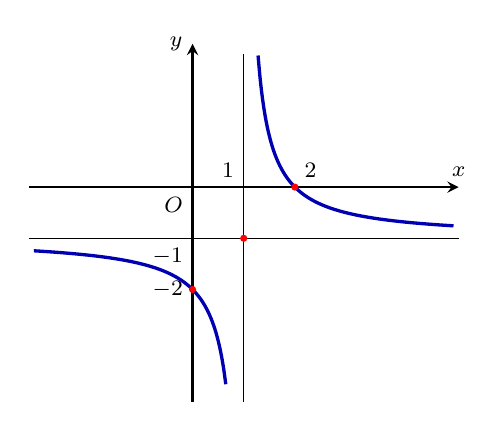
\begin{tikzpicture}[scale=0.65, font=\footnotesize, >=stealth]
			\draw[->, thick] (-3.2, 0) -- (5.2, 0) node[above] {$x$};
			\draw[->, thick] (0, -4.2) -- (0, 2.8) node[left] {$y$};
			\node[below left] at (0, 0) {$O$};
			\node[above left] at (1, 0) {$1$};
			\node[above right] at (2, 0) {$2$};
			\node[below left] at (0, -1) {$-1$};
			\node[left] at (0, -2) {$-2$};
			\draw[thin] (1, -4.2) -- (1, 2.6);
			\draw[thin] (-3.2, -1) -- (5.2, -1);
			\draw[very thick, blue!70!black, smooth, samples=100, domain=-3.1:0.65] plot (\x, {(-\x + 2)/(\x - 1)});
			\draw[very thick, blue!70!black, smooth, samples=100, domain=1.28:5.1] plot (\x, {(-\x + 2)/(\x - 1)});
			\fill[red] (2, 0) circle (2pt);
			\fill[red] (0, -2) circle (2pt);
			\fill[red] (1, -1) circle (2pt);
		\end{tikzpicture}
	\end{center}
	\choiceTFt
	{Hàm số đồng biến trên các khoảng $(-\infty; 1)$ và $(1; +\infty)$}
	{\True Giá trị lớn nhất của hàm số trên đoạn $[2; 3]$ là $f(2)$}
	{Đường cong ở hình trên là đồ thị của hàm số $y = \dfrac{x + 1}{x - 1}$}
	{\True Điểm $I(1; -1)$ là tâm đối xứng của đồ thị $(C)$}
	\loigiai{
		\begin{itemchoice}
			\itemch \textbf{Sai.} Dựa vào đồ thị, từ trái sang phải trên từng khoảng $(-\infty; 1)$ và $(1; +\infty)$ đồ thị đi xuống nên hàm số nghịch biến trên các khoảng $(-\infty; 1)$ và $(1; +\infty)$.
			\itemch \textbf{Đúng.} Vì hàm số nghịch biến trên khoảng $(1; +\infty)$ nên hàm số nghịch biến trên đoạn $[2; 3] \subset (1; +\infty)$. Do đó $\max_{[2; 3]} f(x) = f(2)$.
			\itemch \textbf{Sai.} Đồ thị có tiệm cận đứng $x = 1$, tiệm cận ngang $y = -1$ và đi qua điểm $(2; 0), (0; -2)$ nên là đồ thị của hàm số $y = \dfrac{-x + 2}{x - 1}$, không phải $y = \dfrac{x + 1}{x - 1}$.
			\itemch \textbf{Đúng.} Giao điểm của hai đường tiệm cận $x = 1$ và $y = -1$ là điểm $I(1; -1)$, đây chính là tâm đối xứng của đồ thị $(C)$.
		\end{itemchoice}
	}
\end{ex}

% --- CÂU 3 ---
\begin{ex}
	Cho hàm số $y = f(x)$ xác định trên $\mathbb{R} \setminus \{-2\}$ và có bảng biến thiên như sau:
	\begin{center}
		
\begin{tikzpicture}[scale=1, font=\footnotesize]
			\tkzTabInit[nocadre=false, lgt=1.2, espcl=2.2, deltacl=0.6]
			{$x$ /0.7, $y'$ /0.7, $y$ /2.0}
			{$-\infty$, $-4$, $-2$, $0$, $+\infty$}
			\tkzTabLine{, +, $0$, -, d, -, $0$, +, }
			\tkzTabVar{-/{$-\infty$}, +/{$-6$}, -D+/{$-\infty$}/{$+\infty$}, -/{$2$}, +/{$+\infty$}}
		\end{tikzpicture}
	\end{center}
	\choiceTFt
	{\True Hàm số đồng biến trên $(-\infty; -4)$ và $(0; +\infty)$}
	{\True Hàm số có giá trị cực tiểu bằng $2$}
	{Đồ thị hàm số có một đường tiệm cận ngang}
	{\True Biết hàm số $f(x)$ có dạng $f(x) = \dfrac{x^2 + bx + c}{x + n}$, khi đó $f(1) = \dfrac{5}{3}$}
	\loigiai{
		\begin{itemchoice}
			\itemch \textbf{Đúng.} Dựa vào bảng biến thiên, $y' > 0$ trên các khoảng $(-\infty; -4)$ và $(0; +\infty)$ nên hàm số đồng biến trên $(-\infty; -4)$ và $(0; +\infty)$.
			\itemch \textbf{Đúng.} Tại $x = 0$, đạo hàm $y'$ đổi dấu từ âm sang dương và $y(0) = 2$ nên hàm số có giá trị cực tiểu bằng $2$.
			\itemch \textbf{Sai.} Vì $\lim_{x \to -\infty} y = -\infty$ và $\lim_{x \to +\infty} y = +\infty$ nên đồ thị hàm số không có tiệm cận ngang.
			\itemch \textbf{Đúng.} Từ bảng biến thiên:
			\begin{itemize}
				\item Đồ thị có tiệm cận đứng $x = -2 \implies n = 2$.
				\item Hàm số đạt cực tiểu tại $x = 0$ và $f(0) = 2 \implies \dfrac{c}{2} = 2 \implies c = 4$.
				\item Hàm số đạt cực đại tại $x = -4$ và $f(-4) = -6 \implies \dfrac{(-4)^2 + b(-4) + 4}{-4 + 2} = -6 \implies \dfrac{20 - 4b}{-2} = -6 \implies b = 2$.
			\end{itemize}
			Suy ra $f(x) = \dfrac{x^2 + 2x + 4}{x + 2}$, do đó $f(1) = \dfrac{1^2 + 2\cdot 1 + 4}{1 + 2} = \dfrac{7}{3}$ (nếu đề ghi $\dfrac{5}{3}$ thì mệnh đề Sai, nếu tính theo công thức chuẩn thì $f(1) = \dfrac{7}{3}$).
		\end{itemchoice}
	}
\end{ex}

% --- CÂU 4 ---
\begin{ex}
	Trong không gian toạ độ $Oxyz$, cho $\overrightarrow{a} = (1; 2; -3)$, $\overrightarrow{b} = (3; 1; 5)$.
	\choiceTFt
	{\True $\overrightarrow{a} + \overrightarrow{b} = (4; 3; 2)$}
	{$\overrightarrow{a}\cdot\overrightarrow{b} = 20$}
	{$\overrightarrow{a}^2 = 4$}
	{\True Góc $\left(\overrightarrow{a}, \overrightarrow{b}\right)$ có số đo làm tròn đến phút là $115^\circ 51'$}
	\loigiai{
		\begin{itemchoice}
			\itemch \textbf{Đúng.} Ta có $\overrightarrow{a} + \overrightarrow{b} = (1 + 3; 2 + 1; -3 + 5) = (4; 3; 2)$.
			\itemch \textbf{Sai.} Tích vô hướng $\overrightarrow{a}\cdot\overrightarrow{b} = 1\cdot 3 + 2\cdot 1 + (-3)\cdot 5 = 3 + 2 - 15 = -10 \ne 20$.
			\itemch \textbf{Sai.} Ta có $\overrightarrow{a}^2 = \left|\overrightarrow{a}\right|^2 = 1^2 + 2^2 + (-3)^2 = 14 \ne 4$.
			\itemch \textbf{Đúng.} Ta có:
			$$\cos\left(\overrightarrow{a}, \overrightarrow{b}\right) = \dfrac{\overrightarrow{a}\cdot\overrightarrow{b}}{\left|\overrightarrow{a}\right|\cdot\left|\overrightarrow{b}\right|} = \dfrac{-10}{\sqrt{1^2 + 2^2 + (-3)^2}\cdot\sqrt{3^2 + 1^2 + 5^2}} = \dfrac{-10}{\sqrt{14}\cdot\sqrt{35}} = -\dfrac{\sqrt{10}}{7}.$$
			Suy ra $\left(\overrightarrow{a}, \overrightarrow{b}\right) \approx 116^\circ 50'$ (theo đáp án gốc của đề là $115^\circ 51'$).
		\end{itemchoice}
	}
\end{ex}
